% Copyright (c) 2017-2020 Matematyka dla Ciekawych Świata (http://ciekawi.icm.edu.pl/)
% Copyright (c) 2017-2020 Robert Ryszard Paciorek <rrp@opcode.eu.org>
% 
% MIT License
% 
% Permission is hereby granted, free of charge, to any person obtaining a copy
% of this software and associated documentation files (the "Software"), to deal
% in the Software without restriction, including without limitation the rights
% to use, copy, modify, merge, publish, distribute, sublicense, and/or sell
% copies of the Software, and to permit persons to whom the Software is
% furnished to do so, subject to the following conditions:
% 
% The above copyright notice and this permission notice shall be included in all
% copies or substantial portions of the Software.
% 
% THE SOFTWARE IS PROVIDED "AS IS", WITHOUT WARRANTY OF ANY KIND, EXPRESS OR
% IMPLIED, INCLUDING BUT NOT LIMITED TO THE WARRANTIES OF MERCHANTABILITY,
% FITNESS FOR A PARTICULAR PURPOSE AND NONINFRINGEMENT. IN NO EVENT SHALL THE
% AUTHORS OR COPYRIGHT HOLDERS BE LIABLE FOR ANY CLAIM, DAMAGES OR OTHER
% LIABILITY, WHETHER IN AN ACTION OF CONTRACT, TORT OR OTHERWISE, ARISING FROM,
% OUT OF OR IN CONNECTION WITH THE SOFTWARE OR THE USE OR OTHER DEALINGS IN THE
% SOFTWARE.

\begin{wrapfigure}{r}{5.5cm}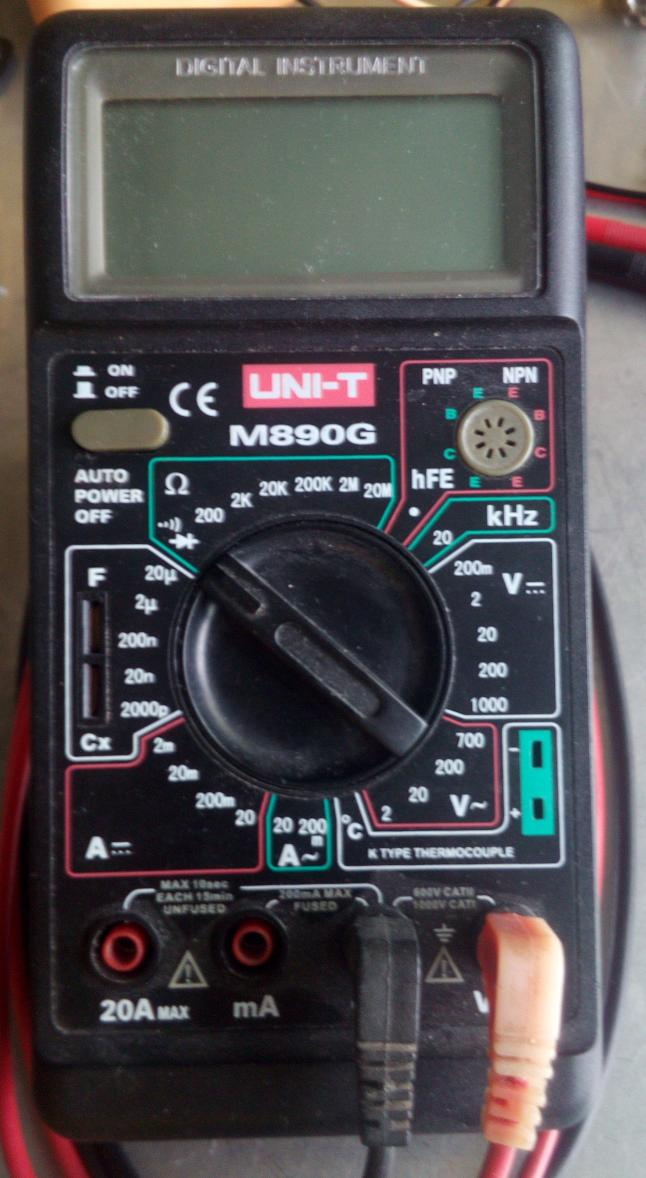
\includegraphics[width=5.5cm]{warsztat_elektroniczny/multimetr}\vspace{-1.2cm}\end{wrapfigure}

\subsection{Multimetr}

Najważniejszym przyrządem w naszym warsztacie elektronika jest uniwersalny miernik parametrów elektrycznych, zwany multimetrem.
Dla naszych potrzeb powinien on zapewniać co najmniej:
\begin{itemize}
	\item pomiar napięcia stałego (DC) od 0.1V do 20V (np. zakresy pomiarowe: 200mV, 20V)
	\item pomiar prądu stałego (DC) od 1mA do 200mA (np. zakresy pomiarowe: 20mA, 200mA)
	\item pomiar rezystancji od 10Ω do 1MΩ (np. zakresy pomiarowe: 200Ω, 20kΩ, 2000kΩ)
	\item pomiar diody
\end{itemize}

\noindent
Przydatne będą także funkcje takie jak:
\begin{itemize}
	\item  sygnalizacja akustyczna ciągłości obwodu (może być razem z pomiarem diody)
	\item pomiar tranzystora "hfe"
\end{itemize}
Oczywiście fajnie jak nasz miernik będzie miał szersze zakresy pomiarowe, będzie umożliwiał pomiar prądu zmiennego (AC), pojemności kondensatorów, itd., ale nie jest to wymagane.

Warto natomiast aby posiadał zabezpieczenie pomiaru prądu (czyli bezpiecznik w tym obwodzie, oznaczenie przy gniazdach "fused") przynajmniej na zakresie do 200mA.
Natomiast przy teście diody warto aby miernik podawał napięcie wystarczające, jeżeli nie do zmierzenia, to przynajmniej do zaświecenia dowolnego LED (czyli tak naprawdę białego lub niebieskiego).
	Niestety producenci na ogół nie podają tego parametru i nawet dobre mierniki potrafią mieć ten paramter zaskakująco słaby.

Ogólnie dobry multimetr jest ważny, ale na początek wystarczy nawet najtańszy model. Jeżeli będziemy kontynuować przygodę z elektroniką to z czasem i tak kupimy drugi, gdyż często przydaje się możliwość równoległego pomiaru w dwóch punktach, równoczesnego pomiaru prądu i napięcia, itd.

Poniżej kilka propozycji do wyboru.

\subsubsection{DT-830B /  DT-830D / DT-832 / DT-832D} (jest wiele bardzo zbliżonych modeli – warto zwrócić uwagę aby miał "fused" na zakresie 200mA oraz buzzer do sygnalizacji ciągłości obwodu)
	\begin{itemize}
		\zaleta spełnia wymagania minimalne oraz posiada pomiar hfe i test ciągłości obwodu
		\zaleta pomiar napięcia DC i AC do 500V
		\zaleta pomiar prądu DC do 10A
		\info od 10PLN
	\end{itemize}

\subsubsection{DT9205A}
	\begin{itemize}
		\zaleta spełnia wymagania minimalne oraz posiada pomiar hfe i test ciągłości obwodu
		\zaleta pomiar napięcia DC i AC do 500V
		\zaleta pomiar prądu DC i AC do 20A
		\zaleta pomiar pojemności
		\info od 20PLN
	\end{itemize}

\subsubsection{DT33A} (nie mylić z DT33B, DT33C i DT33D):
	\begin{itemize}
		\zaleta spełnia wymagania minimalne oraz posiada pomiar hfe i test ciągłości obwodu
		\zaleta pomiar napięcia DC i AC do 500V
		\zaleta pomiar prądu DC do 10A
		\zaleta pomiar pojemności
		\zaleta pomiar temperatury
		\info od 30PLN
	\end{itemize}

\subsubsection{DT890G / M890G / M890C}
	\begin{itemize}
		\zaleta spełnia wymagania minimalne oraz posiada pomiar hfe i test ciągłości obwodu
		\zaleta pomiar napięcia DC i AC do 500V
		\zaleta pomiar prądu DC i AC do 20A
		\zaleta pomiar pojemności
		\zaleta pomiar temperatury
		\zaleta pomiar częstotliwości (tylko DT890G / M890G)
		\zaleta (u niektórych producentów) zabezpieczony pomiar 20A
		\info od 35PLN
	\end{itemize}

\subsubsection{Uni-T UT890C+}
	\begin{itemize}
		\zaleta spełnia wymagania minimalne oraz posiada pomiar hfe i test ciągłości obwodu
		\zaleta pomiar napięcia DC i AC do 500V
		\zaleta pomiar prądu DC i AC do 20A
		\zaleta pomiar pojemności
		\zaleta pomiar temperatury
		\zaleta pomiar częstotliwości
		\zaleta zabezpieczony pomiar 20A
		\zaleta zakresy 6, 60, 600 a nie 2, 20, 200
		\zaleta true RMS
		\info od 76PLN
	\end{itemize}

